\documentclass[UTF8]{ctexart}
\usepackage[left=2cm,right=2cm,top=2cm]{geometry}
\usepackage{amsmath}
\usepackage{enumitem}
\usepackage{float}
\usepackage{threeparttable}
\usepackage{caption}
\usepackage{multirow}
\usepackage{graphicx}
\usepackage{listings}
\usepackage{color}
\definecolor{dkgreen}{rgb}{0,0.6,0}
\definecolor{gray}{rgb}{0.5,0.5,0.5}
\definecolor{mauve}{rgb}{0.58,0,0.82}
\lstset{frame=tb,
  language=C++,
  aboveskip=3mm,
  belowskip=3mm,
  showstringspaces=false,
  columns=flexible,
  basicstyle={\small\ttfamily},
  numbers=left,%设置行号位置none不显示行号
  %numberstyle=\tiny\courier, %设置行号大小
  numberstyle=\tiny\color{gray},
  keywordstyle=\color{blue},
  commentstyle=\color{dkgreen},
  stringstyle=\color{mauve},
  breaklines=true,
  breakatwhitespace=true,
  escapeinside=`,%逃逸字符(1左面的键),用于显示中文例如在代码中`中文...`
  tabsize=4,
  extendedchars=false %解决代码跨页时,章节标题,页眉等汉字不显示的问题
}

\setlength\lineskiplimit{5.25bp}
\setlength\lineskip{5.25bp}

\title{计算方法第七次编程作业报告}
\author{崔士强 PB22151743}
\date{\today}

\bibliographystyle{plain}

\begin{document}

\maketitle

\section{问题描述}
已知质点加速度相对时间的函数,通过Romberg积分求出给定时间的速度,进而求出位置,画出轨迹。
\section{问题分析}
\subsection{Romberg积分}
算法每轮循环对分点的数目加倍,新的数值积分计算只需要依赖上一轮结果和新加入的点处函数值,如此进行直到达到提前设定的
最大迭代次数或达到目标精度。

\subsection{求解方法}
首先对加速度从$1$到$t$积分,得到速度随时间变化的函数,再对这个函数施行Romberg积分,得到位移。

\section{实验结果}
\subsection{结果展示}
\begin{figure}[H]
  \centering
  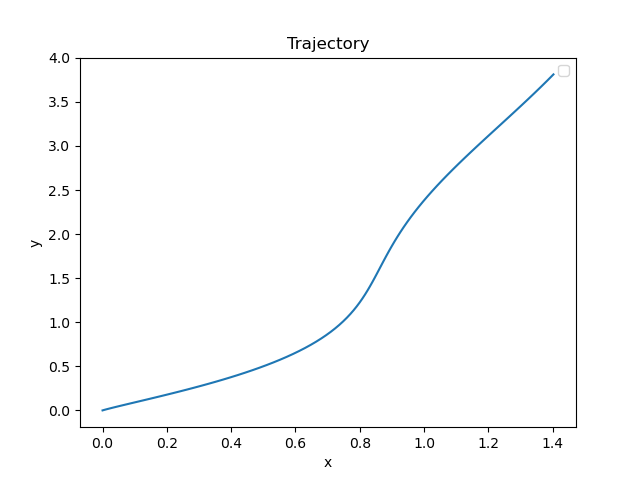
\includegraphics[scale=0.4]{plot.png}
  \caption{轨迹的计算结果}
\end{figure}
\begin{figure}[H]
  \centering
  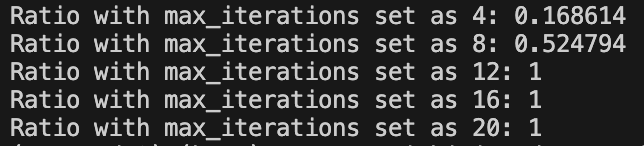
\includegraphics[scale=0.6]{result.png}
  \caption{达到预设精度的比例}
\end{figure}

\subsection{结果分析}
从图2可以看到,随着最大迭代次数的增加,达到预设精度的比例上升,在某一个值后达到1。

最大迭代次数的设置与精度和运行效率直接相关,且二者存在制约。$M$过小可能会导致误差过大,而$M$过大可能会降低
程序运行效率。计算量较大时可以先进行小部分计算,根据达到预设精度的比例调整$M$值。


\bibliography{math}

\end{document}
\iffalse
\begin{figure}[h]
    \centering
    \includegraphics[scale=0.5]{name.png}
    \caption{name}
\end{figure}
\fi
